\section{Theoretische Grundlagen}
    \subsection{Myonen}
        Myonen sind Fermionen und haben demnach einen Spin von $\frac{1}{2}$. Ihre Ladung beträgt -1e, ihre Masse in natürlichen Einheiten \SI{106}{\mega\electronvolt} und ihre Lebensdauer 
        $\tau = \SI{2.2e-6}{\second}$. Die Hauptprozesse zur Erzeugung von Myonen sind die schwachen Zerfälle von geladenen Pionen
        
        \begin{align*}
            \pi^+ \longrightarrow \mu^+ + \nu_{\mu} \\
            \pi^+ \longrightarrow \mu^- + \overline{\nu}_{\mu}
        \end{align*}

        in ein postives oder negatives Myon und das enstprechende Myon-Neutrino. Diese Zerfälle sind ein Folgezerfall von kosmischen Protonen, die in einer Höhe von 15-20km über der Erde in der Atmosphäre
        Pionen erzeuge, welche wiederum um 15km über der Meereshöhe, wie bereits beschrieben, über die schwache Wecheslwrikung in geladene Myonen zerfallen. Während der Propagation der Myonen können auch sie 
        wieder zerfallen. Dies geschieht erneut über die schwache Wecheslwirkung 

        \begin{align*}
            \mu^- \longrightarrow \nu_{\mu} + \text{e}^- + \overline{\nu}_{\text{e}} \\
            \mu^+ \longrightarrow \overline{\nu}_{\mu} + \text{e}^+ + \nu_{\text{e}} 
        \end{align*}

        wobei hauptsächlich Elektronen beziehungsweise Positronen, sowie die entsprechenden Neutrinos dieser und des zerfallenden Myons entstehen. Der Weg den die Myonen bis zu ihrem Zerfall zurücklegen,
        kann für einen auf der Erde ruhenden Beobachter auf zwei Wegen berechnet werden. Angenommen das Myon besitzt eine Energie von E$_{\mu}$\SI{10}{\giga\electronvolt}, berechnet sich die Geschwindigkeit des Myons
        $v_{\mu}$ klassisch über die Gesamtenergie dessen 

        \begin{equation*}
            \text{E}_{\mu}^2 = m_{\mu}^2c^4 + p_{\mu}^2c^2 \qquad \underrightarrow{p_{\mu}=\gamma_{\mu} \text{m}_{\mu}v_{\mu}} \qquad v_{\mu} \approx \num{0.99994}c .
        \end{equation*}

        Daraus ergibt sich über das Weg-Zeit-Gesetz folgende Reichweite

        \begin{equation*}
            \text{s} = v_{\mu} \cdot \tau_{\mu} \approx \SI{658.617}{\metre},
        \end{equation*}

        die keine Myonen auf Meereshöhe erlauben würde. Dass dennoch Myonen detektiert werden, kann durch Einbeziehen der Längenkontraktion gezeigt werden. Demnach haben die Myonen folgende Reichweite

        \begin{equation*}
            \text{s’} = \frac{\text{s}}{\gamma} \approx \SI{60}{\kilo\metre}
        \end{equation*}

        und können auf Meereshöhe detektiert werden. Dies erlaubt auch einen durchschnittlichen Fluss von einem Myon pro \si{\square\centi\metre} pro Minute auf Meereshöhe. Daraus kann die erwartete 
        Ereignisrate in einem Szintillatortank, der als auf dem Boden liegender Zylinder angenommen wird, berechnet werden. Das Volumen des Zylinders entspricht $50\,$l und die Höhe dem zweifachen Radius. So
        lässt sich die Querschnittsfläche parallel zur Erdoberfläche und daraus die erwartete Ereignisrate bestimmen
        
        \begin{equation*}
            \text{Ereignisrate} = \text{h}^2 \cdot \frac{1 \, \text{Myon}}{\si{\square\centi\metre} \cdot \si{\minute}} = \SI{1590}{\square\centi\metre} \cdot \frac{1 \, \text{Myon}}{\si{\square\centi\metre} \cdot \si{\minute}} = \frac{1590 \, \text{Myonen}}{\si{\minute}}
        \end{equation*}

    \subsection{Lebensdauer von Teilchen}
        Die Lebensdauer von Teilchen ist eine mittlere Lebensdauer, da sie angibt, dass 63,2\% aller Teilchen in dieser Zeit zerfallen. Sie lässt sich herleiten, indem angenommen wird, dass innerhalb
        eines infinitessimalen Zeitraums eine Zerfallswahrscheinlichkeit vorhanden ist, die proportional über eine Zerfallskonstante $\lambda$ mit dem Zeitraum zusamenhängt
% \text{A} \cdot \frac{1 \text{Myon}}{\si{\square\centi\metre} \cdot \si{\minute}} =
        \begin{equation}
            \text{dW} = \lambda \text{dt}
            \label{eqn:dW}
        \end{equation}

        Die Anzahl an Teilchen die in diesem Zeitraum zerfallen ergibt sich durch Multiplikation von \eqref{eqn:dW} mit der aktuellen Teilchenzahl N

        \begin{equation*}
            \text{-NdW} = -\lambda \text{Ndt}
        \end{equation*}

        Integrieren und Umstellen dieser Gleichung ergibt das bekannte Zerfallsgesetz
        
        \begin{equation}
            \text{N(t)} = \text{N}_0 \cdot e^{- \lambda \cdot \text{t}}
            \label{eqn:Zerfallsgesetz}
        \end{equation}

        mit der Zerfallskonstante $\lambda$ und den zum Startzeitpunkt vorhanden Teilchen $\text{N}_0$. Die mittlere Lebensdauer lässt sich bestimmen, indem der Erwatungswert der Zeit t aus der zu 
        \eqref{eqn:Zerfallsgesetz} gehörenden Wahrscheinlichkeitsdichtefunktion berechnet wird.

        \begin{equation}
            \tau = \int_0^{\infty} \text{t} \lambda \cdot e^{-\lambda \text{t}} \text{dt} = \frac{1}{\lambda}
            \label{eqn:mittlere_Lebensdauer}
        \end{equation}

        Somit ergibt sich die mittlere Lebensdauer als Inverses der Zerfallskonstante $\lambda$.

    \subsection{Detektion von Myonen}
        Zur Detektion von Myonen können Szintillatoren genutzt werden. Der Konzept der Szintillation beruht darauf, dass einfallende Strahlung Atome des Szintillationsmediums entweder ionisiert oder anregt und 
        diese beim Relaxieren Photonen freisetzen, die detektiert werden. Grundlegend wird zwischen organischen und anorganischen Szintillatoren unterschieden.

            \subsubsection*{Anorganische Szintillatorn}
                Anorganische Szintillationsmedien sind nicht leitende Festkörper, sodass die Eigenschaften der Szintillation von der Gitter- und Bandstruktur des Festkörpers abhängig sind. Da die 
                Szintillationsmedien nicht leiten, liegt eine Energielücke von 4 bis 12 eV zwischen dem Leitungs- und Valenzbands, in der auch die Fermi-Energie liegt. Aufgrund der moderaten Energielücke 
                handelt es sich um Halbleiter, die jedoch noch um ein Lumineszenzzentrum erweitert werden müssen. Diese Zentren sind Bereiche, in denen der Abstand zwischen möglichen Energiezuständen geringer 
                ist als zwischen dem Valenz- und Leitungsband und können entweder durch äußere Dotierung hervorgerufen werden oder sind durch intrinsische Defekte des Mediums bereits vorhanden.
                
                \FloatBarrier

                \begin{figure}[h]
                  \centering
                  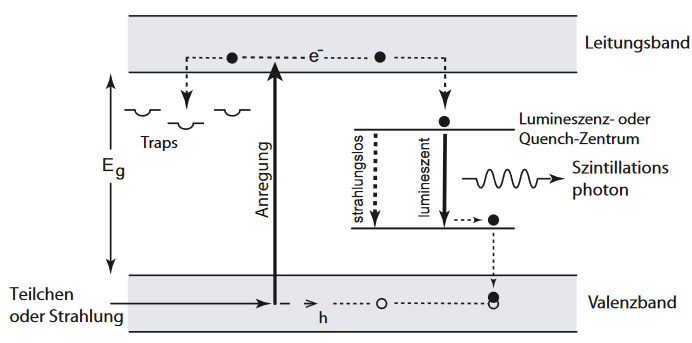
\includegraphics[width = 0.6\textwidth]{pictures/Bandstruktur.png}
                  \caption{In der Abbildung ist die Bandstruktur eines anorganischen Szintillationsmediums, sowie der Ablauf des Szintillationsprozesses abgebildet. Entnommen aus \cite{kolanoski_teilchendetektoren_2016}}
                  \label{fig:Bandstruktur}
                \end{figure}
        
                \FloatBarrier
        
                \noindent

                Wird ein Elektron durch einfallende Strahlung in das Leitungsband angehoben muss es zunächst zum Lumineszenzzentrum wandern. Dieser Weg ist der Grund dafür, dass anorganischen Szintillatoren
                hohe Rückfallzeiten haben und daher weniger zeit-sensitiv als organische Szintillatoren sind. Am Lumineszenzzentrum fällt das Elektron zunächst in den oberen Energiezustand des Zentrums und
                von diesem in den unteren Zustand, bevor es zurück ins Valenzband fällt. Das dabei freigesetzte Photon wird detektiert und hat aufgrund des Übergangs durch das Lumineszenzzentrum eine andere 
                Energie, als die einfallende Strahlung.


            \subsubsection*{Organische Szintillatoren}
                Bei organischen Szintillatoren handelt es sich um organische Moleküle, die immer Kohlenstoff enthalten. Die elektronische Struktur des Kohlenstoffs spielt eine entschiedende Rolle für den
                Szintillationsprozess und ändert sich, sobald das Kohlenstoff in einem Molekül gebunden ist.

                \begin{equation*}
                    \text{C}: \qquad 1\text{s}^2 2\text{s}^2 2\text{p}^2 \qquad \underrightarrow{\text{Molekülverbindung}} \qquad 1\text{s}^2 2\text{s}^1 2\text{p}^3
                \end{equation*}

                In der Molekülverbindung können die s- und p-Orbitale nun unterschiedlich miteinander Hybridisieren. Zu lumineszenten Übergängen kommt es, wenn nur 2 der 3 2p-Orbitale hybridisieren. In diesem
                Fall bleibt ein 2p-Orbital unverändert, das nun die sogenannten $\pi-\text{Elektronen}$ enthält. Die Übergänge dieser $\pi-\text{Elektronen}$ Energieniveaus sind für die Fluoreszenz verantwortlich.
                Da die Elektronen vor dem Zurückfallen auf den Ausgangszustand bereits kleine Übergänge durchlaufen, ist auch hier die Energie der Fluoreszenzelektronen unterschiedlich zu der der anregenden
                Photonen, sodass Erneutanregungen durch Fluoreszenzelektronen vermieden werden. Der Vorteil organischer Szintillationsmedien ist, dass sie auch besonders schnelle Signale zuverlässig 
                detektieren können.

            \subsubsection*{Photoverfielfacher}
                Zur Detektion der Szintillationsphotonen werden Photoverfielfacher genutzt. Sie bestehen aus einer großen Einfalsskathode, aus der einfallende Photonen Photoelektronen auslösen. Diese
                Photoelektronen werden daraufhin durch eine hohe Spannung auf mehrere Dyoden beschleunigt. Bei jedem Auftreffen auf eine Dynode werden zusätzliche Elektronen ausgelöst und es bildet sich 
                folglich eine Lawine an Sekundärelektronen. So kann das Primärelektron um einen Faktor von circa $10^6$ verstärkt und so messbar gemacht werden. Neben der Möglichlkeit bereits ein einzelnes 
                Photon zu detektieren, besitzen Photoverfielfacher auch eine gute Zeitauflösung im  Bereich unter \SI{200}{\pico\second} und eigenen sich daher auch für schnelle Zerfallsprozesse.

                \FloatBarrier

                \begin{figure}[h]
                  \centering
                  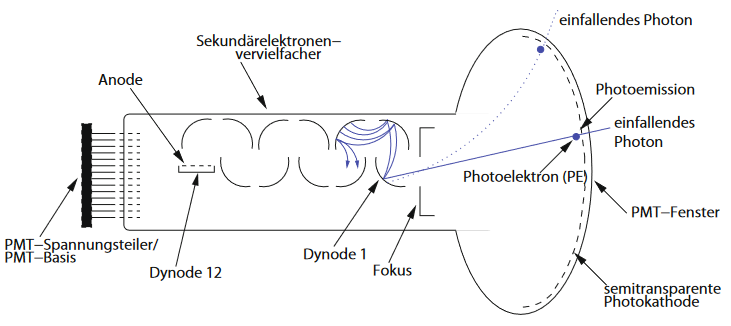
\includegraphics[width = 0.6\textwidth]{pictures/photomultiplier.png}
                  \caption{In der Abbildung ist der schematische Aufbau eines Photonverfielfachers dargestellt. Entnommen aus \cite{kolanoski_teilchendetektoren_2016}}
                  \label{fig:photomultiplier}
                \end{figure}
        
                \FloatBarrier
        
                \noindent 

